\chapter{Analysis}
In this chapter we would like to explain the thinking process before and during the implementation of the back-end application. We are going through individual parts from the back-end application requirements, explaining problems associated with them and revealing what possibilities we had to solve them and how we decided in the end.

\section{General problems}
\subsection{Authentication}
In our application we had to deal with authentication for customers and employees. There are many ways how users can be authenticated in API. We ended up with token authentication - in each request clients must set the Authorization header with the token. Client can get the token in exchange for correct credentials.

Another part of the authentication we consider in the analysis is at least the basic security during the manipulation with auth data and flawless verifying token sending.

\subsubsection{Token authentication details}

We decided to implement it on our own, using only Rails helpers for generating and verifying secure tokens. As you can see in \ref{auth-token-scheme}, token is generated during the login action and then returned in body of the response. All the following requests must have this token in it's header to be authenticated.

\begin{figure}[h]\centering
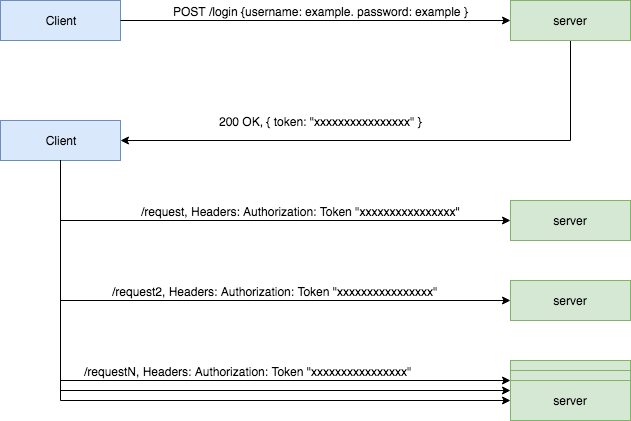
\includegraphics[width=\textwidth]{auth/Auth.png} 
\caption{Auth token scheme}\label{auth-token-scheme}
\end{figure}

Our application store just one token per user. That implies the user can be logged in from one device at time only. Having more valid token for users would let into several problems with invalidating them in case of log out and also this approach has one advantage. If someone reveals user credentials and log in with them - user will know that in the moment it tries to use the app, because all it's requests would be unauthenticated.

In Ruby on Rails there exists very good gem for authentication - \textit{devise\_token\_auth} \footnote{\url{https://github.com/lynndylanhurley/devise\_token\_auth}} which we half-implemented at first. However we decided to not use it in the end. Main reason for not using it was - at the time of writing the authentication part - very unstable and badly documented front-end library part. More details about problems we came across during the analysis/implementation in the next paragraph.

First reason for not using the gem was, that it uses email as main default authentication field. For customers we wanted to use the telephone number as the main identifier - including the SMS confirmation and password recovery (explained later), which would led us to rewrite the most of the gem's controllers and models anyway and as bonus we would have to integrate it with the existing parts of gem.

Second reason was the complexity of the whole authentication process. This gem would bring to our project more secure but also much more complex way of authenticating. Once client gets the token from the login endpoint, the token is generated and returned with each following request. Using this approach we have to solve the batch request problem. Imagine that client sends for example three requests at once to the server. Of course all the three requests must have same authentication token - because client doesn't have the new token until the response comes. Thus server must accept all those three requests as authenticated, but also they must agree with the front-end which response has the correct new auth token - responses don't have to come in order in which they were sent. This complicated process was implemented in the back-end gem and couldn't be changed. The front-end library was supposed to implement that, but after the three weeks of trying and founding several bugs in the library - even without successful login they gave up using it.

In conclusion if we had wanted to use the gem on backend we would have to understand the whole gem auth process in detail and specify it for the front-end. Front-end would then have to write the whole complicated solution on their own. 

We came to conclusion that the complexity, that would bring this library to our application is not worth the better security and stability we would gain from this. Using HTTPS on both server and client makes the token theft little bit harder - so lack of this generation process with each request is not a big deal. Also the only really sensitive accounts for identity theft are the employees one's and we are in personal contact with them, so we would know about misuse or potential hack and we could provide the safer solution later.

\subsubsection{Basic security}
As we mentioned in last paragraphs, our token solution is not perfect from the security perspective. Besides the token (which could be easily rewritten more securely in the future ) we tried not to take the security of our application lightly.

First of all, we don't store passwords in plaintext. We use Rails integrated feature \textit{has\_secure\_password}\footnote{\url{https://api.rubyonrails.org/classes/ActiveModel/SecurePassword/ClassMethods.html}}, which uses BCrypt hash function.

Thanks to the Ruby on Rails framework we also excerpt passwords from the logs and we are not vulnerable to SQL Injection\footnote{\url{https://en.wikipedia.org/wiki/SQL\_injection}}.

\subsubsection{Sending verifying tokens}
We must send tokens via emails and SMS during the whole authentication process. Because these are actions that are not instant (API request, SMTP request) and because in Rails we can easily create asynchronous workers, we decided to have these functions handled as Sidekiq workers. In exchange for some time spent on configuration we have instant response without blocking webserver threads during account creation/recovery and have ability to automatically resend the message in case of the third party or network failure.

\subsection{Authorization}
Almost every endpoint has it's own rules of who and in what circumstances can do such action. There are two main groups of users - employees and customers. Employees are then divided into three groups - administrators, drivers and dispatchers. There are just two types of customers - registered and unregistered. Each visitor is one of these types.

In each request we have to solve specific condition whether current user is able to do this action or not. Having the all these conditions directly in controllers would make the controllers difficult to read. Also these conditions could change in the future and have changed during the development several times. This led us to have the authorization conditions separated in the different part of the application.

We want to avoid reinventing the wheel so we have chosen to use for such purpose \textit{Pundit} \footnote{\url{https://github.com/varvet/pundit}} gem. 

Another option we looked into was \textit{Cancancan} \footnote{\url{https://github.com/CanCanCommunity/cancancan}} gem. They both have long maintenance history, are actively developed in the time of writing and satisfies all of our conditions for the authorization. Cancancan is better suited for applications with complicated views, because it provides more helpers for checking authorization in them. Also its architecture is more general thus it is better optimized for more complicated permission management. That results in slightly more complex permission definitions. On the other side pundit is more light-weight solution with very simple architecture and permissions definition files. Because our permissions are not complicated very much and we wanted to have them written as simply as possible, this was the main reason why we chose Pundit over Cancancan.

 \subsection{Pagination}
 paginating lists - why, where
\subsection{Request parameters security}
Permiting

\subsection{Rendering views}
\subsection{Localization}
- more languages - errors
 - we translate on our side, frontend on its => bad pattern
\subsection{Images}
	- too difficult for front-end to implement and handle api multipart requests
	- limitation only one image for entity => but enough for us
	- employee and vehicle images


\section{Customers}
Use email as main distinguishing field is kind of standard in web authentication. We came to the conclusion that we should use as our identifier telephone number. Despite the standard and the the consequence of this decision - lack of any easy to use library for authentication in Rails. Reasons which led us to this decision:
\begin{itemize}
	\item During the order process we must be able to contact customer immediately in case of emergency, so we need the customer's phone anyway.
	\item Customers are going to register mostly from their phones. That phone can receive SMS for sure - not everyone has direct access to his mail from phone. 
\end{itemize}
\subsection{Create and confirm}
Besides the authentication and params problems \todo{give links} described in general problems section we also have to to deal with the telephone verification.

We decided to use verification via SMS code.

 Registered telephone number must be verified.  Before the customers can do so, they must go through telephone number confirmation process as follows: Customers receive SMS with registration token. This token is valid for 5 minutes and customer can ask for resend.  Resend will invalidate last token, generate new and send it. Confirm is made with provided token and telephone number.
 
 Based on requirements we decided to split these functions into three API endpoints - \textit{create}, \textit{confirm} and \textit{resend\_confirmation}.
 
 \subsection{Password recovery}
 Whole password recovery procedure is similar to the create account one.
 Based on specification we split the password recovery feature into two API endpoints - \textit{password\_recovery} and \textit{reset\_password\_by\_token}. 
 
 Calling first endpoint - password recovery - sends in exchange for the telephone number SMS to that telephone number with password recovery token. Then the customer can send request with this token, his telephone number and a new password - which if all the conditions are satisfied - will be set. 
 
 The token consists of 4 numbers and is valid for 5 minutes. This parameters we just picked as similar to the others services on the internet and of course we must be able to change them later if we discover that it's not good.
 
 During the analysis we have noticed, that the first endpoint must except the bad request format always return success status. Especially, we can not let the client know whether the account with such telephone number was not found and neither that the SMS was not sent successfully. If we would return error code in such situation, someone could potentially get the telephone numbers for all of our customers.
 
 Also we are aware that the SMS may not be the most secure way of verifying users\footnote{\url{https://www.cnet.com/how-to/why-you-are-at-risk-if-you-use-sms-for-two-step-verification/}} but we think that at our scale, potential losses for stolen customer's account wouldn't be crucial - there is no credit system or something valuable on the account. The worst case is that the attacker orders a taxi on victims name and thus that order will be fraud - which happens few times a week now anyway.
 
 \subsection{Favourite places}
 We decided to have an endpoint with four parameters, which will return the list of N recommended places ordered from the most to the least appropriate.
 
 First is parameter is the maximum number of places we would like to receive, second is customer id for whom we want to have recommendations for, third is the location and the last - 'start' - parameter  says one of the following:
 \begin{itemize}
 	\item true = we want recommendations for pick-up places and the provided location are customer's current coordinates
 	\item false = we want recommendations for drop-off locations and the provided location are pick-up coordinates
 \end{itemize}
 
 Our first problem to solve was how to handle locations from the request. We suppose that the location which goes to our API is directly from the customer's telephone sensors, thus there's nothing like Example's restaurant official coordinates, which would client sent to us whenever he wants taxi from that restaurant. On the other hand, we would like to group all these locations near the Example restaurant into one place, so we can recommend it just once and there was enough space for other interesting places. We thought about using some kind of modified clustering algorithm but we ended up with conclusion that this would be in our case overkill. We came to conclusion that for our use case is enough to have defined distance constant and all the places around this place within the constant distance are considered as one place. We set this constant to 50 meters, because it seems like good compromise between inaccurate low-end phones GPS precision and the distance between two different places. Of course that we must be able to change this constant in the future if we discover, that it is too small or big.
 
 Second problem was how to filter and return the list of places fast. For each user we have index of visited places with information on which we base our recommending algorithm. In this index we have following information about each place:
 \begin{itemize}
 	\item coordinates
 	\item list of items containing for each place occurrence in orders:
 	\begin{itemize}
 		\item decimal number from 0 to 1 which says, how long ago was order with this place placed. 1 has user's last order and 0 has user's furthermost order .
 		\item time-stamp when was the order created
 		\item start = whether was the place in the order used as a start or finish
 	\end{itemize}
 	\item list of corresponding places (drop-off for pick-up and vice versa).
 \end{itemize}
For the given parameters in request, we go in index place by place and count the weight of it from the occurrences weights multiplied by constant if start/finish fits the desired direction. Index is also prepared for recommending places based on the order time (e.g. in the evening we go to pub, in the morning to work). We decided to limit the recommendation index for last 1000 orders for each user.

In our research we haven't found any ready-made solution for this problem, so we decided to come up with our own solution. Of course it could be more effective and recommendation could be done even smarter. During the development we came to this algorithm which satisfies all our specified metrics and thus we were satisfied with the application of it in the real world.


\section {Orders}
Format of times
Cost of api requets, Google API
order planning system
\begin{figure}[h]\centering
	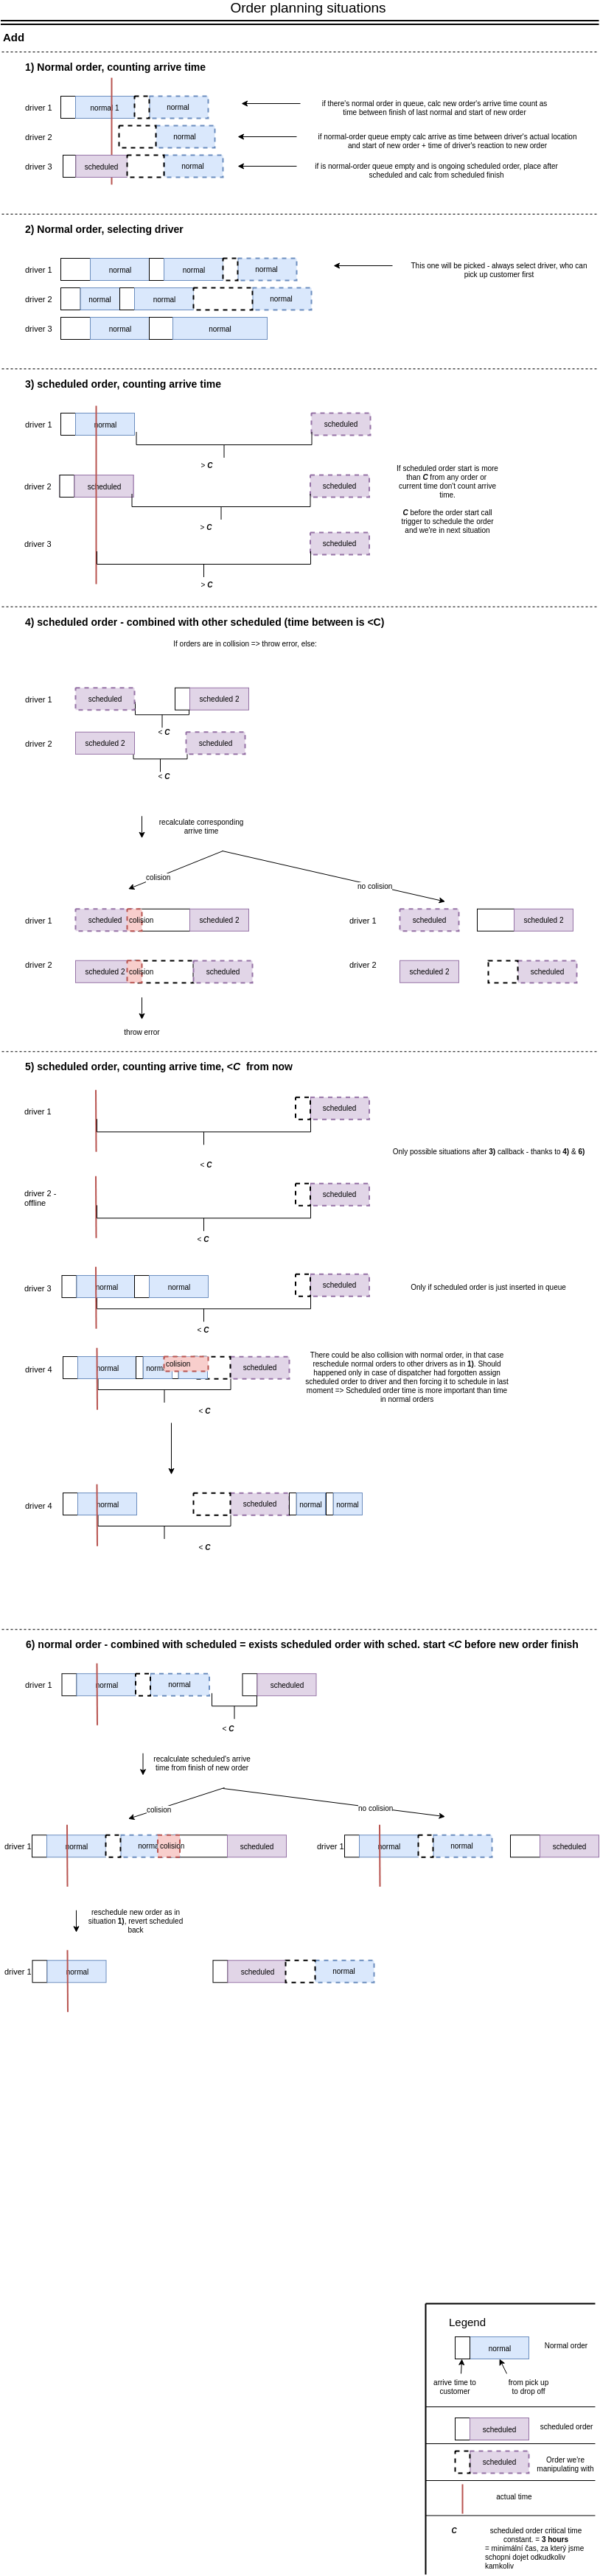
\includegraphics[scale=0.2	]{orders/order_planning.png}
	\caption{Order planning situations}\label{order-process-scheme}
\end{figure} 
